\documentclass[12pt]{article}
\usepackage[francais]{babel}
\usepackage[utf8]{inputenc}
\usepackage{graphicx}
\usepackage{amsmath}
\usepackage{amsfonts}
\usepackage{amssymb}




\addtolength{\hoffset}{-1cm}
\addtolength{\textwidth}{2cm} 
\addtolength{\voffset}{-1cm}
\addtolength{\textheight}{2cm} 

\begin{document}

\begin{titlepage}
\begin{center}

\hfill
\vfill
\bigskip
\huge{ 
\includegraphics[width=60,height=50]{logo.png} 

\includegraphics[width=80,height=50]{lh.png} \\
 Rapport de stage \\ M2 MATIS  \\ \\ \\ \\ \\
 } 
\vfill
\bigskip 
\Huge 
\bigskip 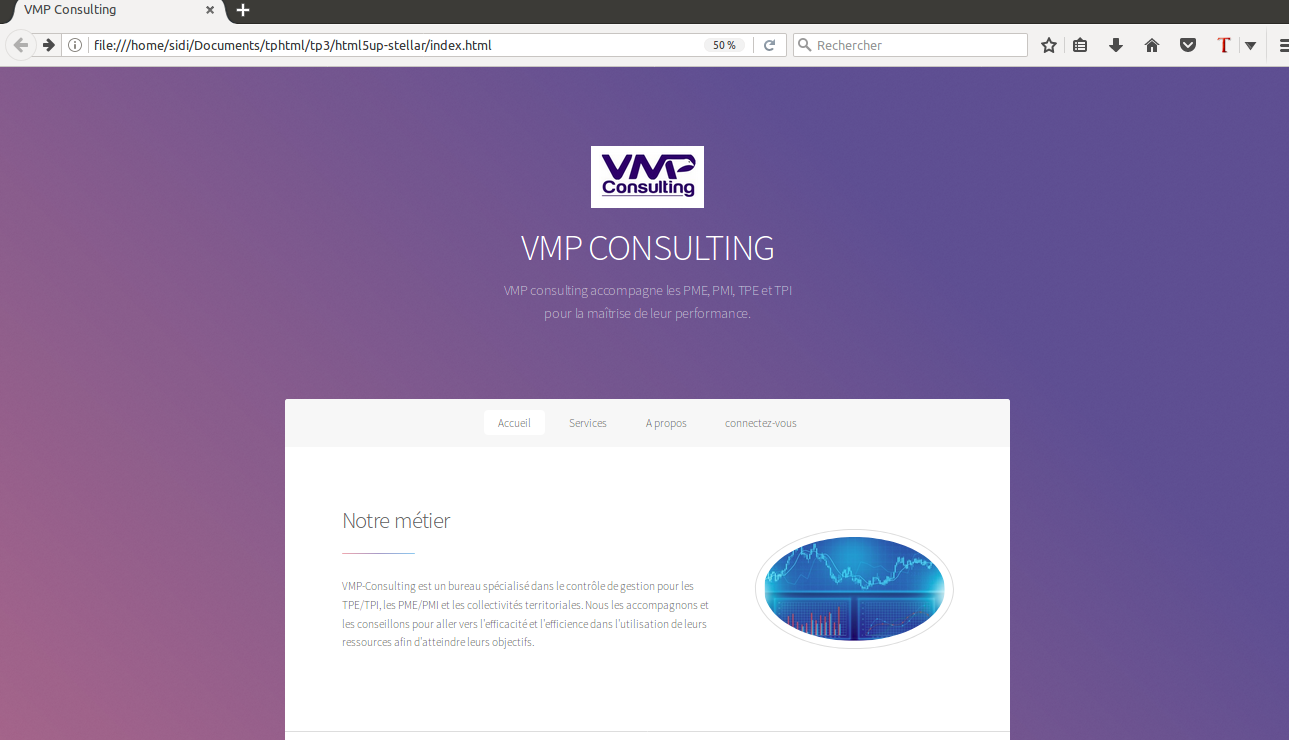
\includegraphics[width=120,height=150]{design1.png}} \\ \\
 Développement d'un portail web pour VMP Consulting \par 
\vfill

\Large \begin{flushleft}
 Réalisé par:\\ sidi Maouloud \par
\end{flushleft}
		 
		  \begin{flushright}
		                    sous la direction de:\\  M. ould Maouloud
		                   \end{flushright}



		 
\vfill
\Large Université du Havre \par \Large VMP Consulting		
		\bigskip 
\bigskip

\Large
28 Octobre 2017
\end{center}
\end{titlepage}

\section*{Remerciements}
Premièrement, je tiens á transmettre ma gratitude et mon affection à ma mère, mon père  et ma
sœur, ainsi que mes proches pour leur patience et leur soutien.\\ \\

J’adresse tout d’abord mes remerciements à  M. sidi ould MAOULOUD, de m’avoir accueillie pour faire mon
stage au sein de son entreprise, ainsi pour son aide et  ses  remarques pertinentes.  \\ \\
J’aimerais aussi remercier M. Laurent Amanton  et tous mes enseignants de l’université du havre
qui m’ont accompagné 
au cours de cette année.\\ \\


\newpage

\section*{Résumé}
VMP-Consulting est un bureau spécialisé dans le contrôle de gestion pour les TPE/TPI, les PME/PMI et les collectivités territoriales. Il les accompagnons et les conseillons pour aller vers l'efficacité et l'efficience dans l'utilisation de leurs ressources afin d'atteindre leurs objectifs.\\
Pour mieux servir ses clients, VMP Consulting veut avoir un portail web pour 
mettre en œuvre un espace de travail unique pour les clients, 
 proposer aux clients un accès privilégié et personnalisé à divers services en
ligne, et 
développer des outils qui permettent aux clients de réagir avec les contenus du
portail.\\
L'objectif de ce stage est de réaliser ce site web.


\section*{Abstract}
Whatever the activity, today all companies are confronted with increased competitive pressure, technological changes ... To enable managers and operational staff to devote themselves entirely to their core business, support in managing The company is a necessity not to say an obligation. In this area, not all businesses are housed in the same category, particularly small businesses and small businesses. The lack of management tools is mainly linked to a problem of means although sometimes it can be a problem of awareness of the utility and the benefit brought by these tools.\\
VMP-Consulting is an office specializing in management control for small and medium-sized enterprises (SMEs), SMEs and local authorities. He accompanies them and advises them to move towards efficiency and efficiency in the use of their resources in order to achieve their objectives.

\newpage

\tableofcontents
\newpage



\section{Introduction et Problématique}

\subsection{VMP Consulting}
VMP-Consulting est un bureau spécialisé dans le contrôle de gestion pour les TPE/TPI(trés petite entreprise), les PME/PMI(petite moyenne entreprise) et les collectivités territoriales. Il les accompagne et les conseille pour aller vers l'efficacité et l'efficience dans l'utilisation de leurs ressources afin d'atteindre leurs objectifs.\\ \\

Quelle que soit l’activité, aujourd’hui toutes les entreprises sont confrontées à une pression concurrentielle accrue, aux évolutions technologiques...Pour permettre aux managers et aux opérationnels de se consacrer entièrement à leur coeur de métier, un accompagnement dans la gestion de l'entreprise est une nécessité pour ne pas dire une obligation. Dans ce domaine là, les entreprises ne sont pas toutes logées à la même enseigne, en particulier les TPE et certaines PME. Le manque d’outils de gestion est principalement lié à un problème de moyens même si parfois il peut s’agir d’un problème de sensibilisation à l’utilité et le bénéfice apporté par ces outils.\\ \\
VMP consulting accompagne les PME, PMI, TPE et TPI pour la maîtrise de leur performance, avec ses solutions, pour atteindre les objectifs de :
\begin{itemize}

\item Maîtriser les coûts.

\item Optimiser les performances.

\item Une transparence sur la gestion des ressources de  l'entreprise.

\item Le développement de la réactivité dans la prise de décisions stratégiques.
\end{itemize}
\\ \\ 
Le créateur du startup a une expérience de plus de 20 ans dans divers secteurs d'activités et dans plusieurs types de structures (PME - Multinationales - Organismes d'Etat), et en 2016 


\subsection{Problématique}

\subsection{Objectifs et Cahier de charges}

\newpage

\section{Analyse et Conception}

\subsection{Modélisation}

\subsection{Bases de Données}

\subsection{Front-end}

\subsection{Banck-end}

\subsection{Outils}

\newpage

\section{Développement et Implémentation}

\subsection{Symfony}

\subsection{Dashboard}

\subsection{Temps réel}

\newpage

\section{Résultats et Tests}

\subsection{Démonstrations}

\subsection{Tests}



\newpage
\section{Conclusion}


\newpage
\section{Bibliographie}


		
\end{document}
